% Relatório da versão 1 do software ipump para o curso
% Sistemas de Controle - DCA0206 - UFRN
% Autores:
%   AUGUSTO MATHEUS PINHEIRO DAMASCENO
%   MARCEL DA CÂMARA RIBEIRO DANTAS
%   PABLO HOLANDA CARDOSO
%   PEDRO DE CASTRO GURGEL LIMA
%   RODRIGO DANTAS DA SILVA
% Modificado por: Ícaro Bezerra Queiroz de Araújo
%

%%%%%%%%%%%% STRUCTURE %%%%%%%%%%%%%%%
\documentclass[a4paper,12pt]{article}
\usepackage[T1]{fontenc}
\usepackage[utf8]{inputenc}
\usepackage[brazil]{babel}
\usepackage{lmodern}
\usepackage{setspace}
\usepackage[top=2cm, bottom=2cm, left=2cm, right=2cm]{geometry}
%%%%%%%%%%%%%%%%%%%%%%%%%%%%%%%%%%%%%%

%%%%%%%%%%%%%%%% PAGES STYLE %%%%%%%%%
\usepackage{fancyhdr}
\fancypagestyle{main}{
\renewcommand{\headrulewidth}{0pt}
\fancyhead[RO]{\thepage}
\fancyfoot[CO]{}
}
%%%%%%%%%%%%%%%%%%%%%%%%%%%%%%%%%%%%%%

\usepackage{graphicx}
\usepackage{float}
\usepackage{epstopdf}
\usepackage{subfig}
\usepackage{mathptmx}
\usepackage{changepage}
%\usepackage[alf]{abntex2cite}

%%%%%%%%%%% PDF METADATA %%%%%%%%%%%%%
\usepackage[ pdftitle={MODELO RELATÓRIO},
pdfsubject={INTRODUÇÃO AO LABORATÓRIO DE CONTROLE - Grupo 3},
pdfkeywords={Controle,Automação,UFRN,DCA,ipump},
hidelinks]{hyperref}
%%%%%%%%%%%%%%%%%%%%%%%%%%%%%%%%%%%%%%

\begin{document}

\onehalfspacing

\thispagestyle{empty}

\setcounter{page}{1}

%%%%%%%%%%%% LOGOS %%%%%%%%%%%%%%%%%%%

\begin{figure}[!ht]

\centering

\subfloat{

\includegraphics[width=2.7cm]{UFRN.eps}
\label{UFRN Logo}
}
\hspace{11.09cm}
\subfloat{

\includegraphics[width=2.4cm]{DCA.eps}
\label{DCA Logo}
}

%\caption{}
\label{Logos}

\end{figure}

%%%%%%%%%%%%%%% CAPA %%%%%%%%%%%%%%%%%

\vspace{-1cm}

\begin{center}
{\bf{\normalsize UNIVERSIDADE FEDERAL DO RIO GRANDE DO NORTE\\
CENTRO DE TECNOLOGIA\\
DEPARTAMENTO DE ENGENHARIA DE COMPUTAÇÃO E AUTOMAÇÃO\\
CURSO DE ENGENHARIA DE COMPUTAÇÃO
}}


\vspace{3.6cm}

{\bf{\large RELATÓRIO DA 1ª EXPERIÊNCIA\\
INTRODUÇÃO AO LABORATÓRIO DE CONTROLE\\
}}
\vspace{1.5cm}
{\large TURMA: 01 A\\
	GRUPO Nº}

\vspace{3.6cm}



\begin{flushright}
\begin{normalsize}
ANDRESSA STÉFANY SILVA DE OLIVEIRA: 20160154101\\
\vspace{0.8cm}
FERNANDA MONTEIRO DE ALMEIDA: 20160154228\\
\vspace{0.8cm}
VITOR RAMOS GOMES DA SILVA: 20160154415\\
\vspace{0.8cm}
MÁRCIO LUIZ BEZERRA LOPES JÚNIOR: 20160154326\\
\end{normalsize}
\end{flushright}


\vspace{2.5cm}

{\large Natal-RN\\
2017}

\end{center}

\newpage

%%%%%%%%%%%%%%%  CONTRA-CAPA %%%%%%%%%

\thispagestyle{empty}

\begin{center}
\begin{normalsize}
ANDRESSA STÉFANY SILVA DE OLIVEIRA: 2016015410\\
\vspace{0.8cm}
FERNANDA MONTEIRO DE ALMEIDA 20160154228\\
\vspace{0.8cm}
VITOR RAMOS GOMES DA SILVA: 20160154415\\
\vspace{0.8cm}
MÁRCIO LUIZ BEZERRA LOPES JÚNIOR: 20160154326\\

\end{normalsize}
\end{center}
\vspace{3cm}

{\bf{\large {\centering INTRODUÇÃO AO LABORATÓRIO DE CONTROLE\\}}}

\vspace{4cm}

\begin{adjustwidth}{7.5cm}{0cm}

{\normalsize

Primeiro Relatório Parcial apresentado à disciplina de
Laboratório de Sistemas de Controle, correspondente à
avaliação da 1º unidade do semestre 2017.1 do 8º período
do curso de Engenharia de Computação da
Universidade Federal do Rio Grande do Norte, sob
orientação do {\bf Prof. Fábio Meneghetti Ugulino de
Araújo.}

}

\end{adjustwidth}

\vspace{2cm}

\begin{center}

Professor:  Fábio Meneghetti Ugulino de Araújo.

\vspace{2.5cm}

{\large Natal-RN\\
2017}

\end{center}

\newpage

%%%%%%%%%%%%%%%  RESUMO %%%%%%%%%%%%%%

\thispagestyle{empty}

\begin{center}
{\large \textbf{RESUMO}}
\end{center}

\vspace{3cm}

\begin{flushleft}

\hspace{4ex}O presente trabalho é referente ao desenvolvimento de um software que se comunica com um sistema de tanques, uma planta Quanser, e seu simulador, o qual possui canais para leitura e escrita de sinais. Primeiro, houve a análise matemática das relações entre vazão de entrada, vazão de saída, tensão enviada para a bomba e o nível de água presente no tanque. Além disso, o sistema possui duas situações: malha aberta, a qual o usuário escolhe a tensão a ser enviada; e malha fechada, nesse caso, o usuário indica exatamente o nível que a água deve estar. O usuário também escolhe o tipo de sinal que está sendo enviado (degrau, onda quadrada, entre outros). Posteriormente, fazendo uso de dados adquiridos experimentalmente, obteve as equações referente ao comportamento do fluxo da água com relação à bomba, como também, a associação da altura com a tensão. O comportamento do sistema é informado para o usuário através de gráficos presentes na interface do software, tanto o sinal de entrada escolhido como os valores que são lidos nos canais indicados pelo usuário.\\

\end{flushleft}

\vspace{1.5cm}

\textbf{Palavras-chave:} sistema de tanques; sistema de controle; software; planta Quanser.

\newpage

%%%%%%%%% LISTA DE FIGURAS %%%%%%%%%%%

\thispagestyle{empty}

\begin{center}
\listoffigures
\end{center}

\newpage

%%%%%%%%%%%%%%% SUMÁRIO %%%%%%%%%%%%%%

\thispagestyle{empty}

\begin{center}
\tableofcontents
\end{center}

\newpage

%%%%%%%%%%%%%%% INTRODUÇÃO %%%%%%%%%%%

\thispagestyle{main}

\section{INTRODUÇÃO}

\begin{flushleft}
\hspace{4ex}A introdução serve para o leitor ter uma noção genérica do tema que será
abordado. Uma boa introdução deve criar uma expectativa positiva no leitor e despertar
seu interesse pela leitura do restante do trabalho. Deve apresentar, basicamente, a
delimitação do assunto o(s) objetivo(s) do estudo e sua finalidade, o ponto-de-vista sob
qual o assunto será tratado, enfim, os elementos necessários para situar o tema do
trabalho.
\end{flushleft}

\newpage

%%%%%%%%%% REFERENCIAL TEÓRICO %%%%%%%

\thispagestyle{main}

\section{REFERENCIAL TEÓRICO}

\subsection{MODELAGEM}
\hspace{4ex}O sistema a ser controlado é representado pelo seguinte sistema.
\begin{figure}[h]
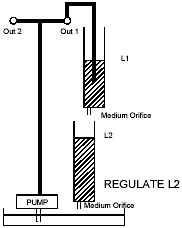
\includegraphics[scale=1]{tanques.png}
\caption{Sistema de tanques}
\label{fig:tanques}
\end{figure}

\hspace{4ex}Sabemos que a vazão de entrada é dada por $ k_mu(t) $ e a vazão de saída $ \sqrt{2gh(t)}a $, onde $k_m$ é a constante da bomba e $"a"$ a área do orificio. Assim: 
\[ \frac{dq}{dt}=qin-qout\]
\[ A\frac{dh(t)}{dt}=k_mu(t)-\sqrt{2gh(t)}a \]
\[ A\frac{dh(t)}{dt}=k_mu(t)-\sqrt{2gh(t)}a \]
\[ \frac{dh(t)}{dt}= \frac{k_m}{A}u(t)- \frac{a\sqrt{2gh(t)}}{A} \]

\subsection{ANALISE}
\hspace{4ex}Para atingir um certo nível no tanque estamos interessados no valor de tensão que fará o sistema alcançar esse nível. Para isso precisamos analisar o regime permanente. Após algum tempo a altura praticamente não vai mais variar, então podemos considerar.  $\frac{dh(t)}{dt}=0 $, com isso nossa equação fica:
\[ \frac{k_m}{A}u(t)= \frac{a\sqrt{2gh(t)}}{A} \]
\[ u(t)=  \frac{a\sqrt{2gh(t)}}{k_m}\]
\begin{equation}\label{eq:1}
u(t)=k\sqrt{h(t)}
\end{equation}
\hspace{4ex}Por questões de simplificação e como a variação da altura é pequena, aproximamos para uma função linear. Com a relação do sinal de entrada com o nível final do tanque, podemos calcular experimentalmente o valor de k, aplicando um sinal de entrada do tipo degrau e observando o seu valor final.
Com o valor de k calculado, dado um nível sabemos qual a tensão necessária para atingi-lo.

\subsection{SENSORES}
\hspace{4ex}Para obter o nível dos tanques são utilizados sensores de pressão. a saída desses sensores são uma tensão proporcional a pressão e como a pressão é proporcional a altura podemos encontrar uma relação linear da tensão com a altura da água.


\subsection{SISTEMA EM MALHA ABERTA}
\begin{figure}[H]
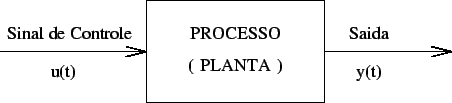
\includegraphics[width=15cm]{malhaAberta.png}
\caption{Malha aberta}
\label{fig:malhaAberta}
\end{figure}
\hspace{4ex}No processo em malha aberta não existe nenhum controle o sinal de entrada é a tensão e a saída o nível do tanque que é lida pelo sensor.


\subsection{SISTEMA EM MALHA FECHADA}
\hspace{4ex}No processo em malha fechada o sinal de entrada é o nível de referência.
A entrada do controlador é a diferença de nivel desejado para o medido, a saida do controlador é a própria diferença somada com a tensão necessária para o sistema estabilizar naquele nível, utilizando a equação \ref{eq:1}.
Assim a tensão somada dá o valor necessário para estabilizar e o erro acelera esse processo.
O período de amostragem e o controle do sistema é feito a cada 100 milisegundos.


\begin{figure}[H]
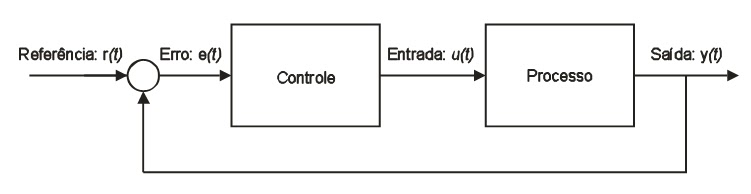
\includegraphics[width=15cm]{malhaFechada.jpg}
\caption{Malha Fechada}
\label{fig:malhaFechada}
\end{figure}


\newpage

%%%%%%%%%% METODOLOGIA %%%%%%%%%%%%%%%

\thispagestyle{main}

\section{METODOLOGIA}


\hspace{4ex}Neste sistema de controle desenvolvido, foi utilizado a planta da \textit{Quanser}, um sistema com dois tanques com altura de 30cm e diâmetro de 4,45cm cada. Desejava-se controlar o nível dos tanques com a bomba através das tensões enviadas para a uma placa onde havia uma comunicação cliente-servidor. Fez-se um experimento inicial para se ter conhecimento do comportamento do fluxo de água enviado pela bomba, a vazão de saída dos tanques e a leitura dos sensores. Assim como os níveis de equilíbrio entre a vazão de entrada e saída. Após a obtenção desses valores, comparou-se com as constantes obtidas na documentação do fabricante: constante da bomba e constante para conversão dos valores obtidos do sensor para centímetro. Foi adotado, então, a constante do  sensor do fabricante na conversão das leituras recebidas do sensor. Não foi necessário a constante da bomba, apenas para simulações feitas sem o uso da planta.

Em seguida, foi feito o planejamento do leiaute do software de controle, os parâmetros de entrada e os valores de saída a serem apresentados nos gráficos, seguindo as especificações do roteiro. O programa foi feito no ambiente Qt Creator utilizando a linguagem C++, pois tinha suporte para interface gráfica. A leitura e escrita não foi paralelizada para evitar alguns conflitos de sincronização. 

Após finalizado o sistema, a validação do controle foi feita testando cada função de entrada: degrau, senoidal, dente de serra e aleatório. Variando também os valores de entrada e fazendo a comutação entre malha fechada e aberta. 

No caso específico da malha fechada onde seria necessário utilizar as leituras do sensor, foi utilizado a seguinte estratégia: a referência era enviada para a placa e ao receber as leituras do sensor, esses valores eram comparados. Se houvesse alguma diferença, ou erro, era corrigido na referência diminuindo-se o erro.


\newpage

%%%%%%%%%% RESULTADOS %%%%%%%%%%%%%%%

\thispagestyle{main}

\section{RESULTADOS}

\hspace{4ex}

\subsection{Programa de controle}
O sistema no geral não apresentou problemas de conexão com o servidor, como perda de conexão ou atrasos consideráveis nos dados recebidos. Para o caso de não paralelizar a leitura e escrita de dados, foi observada que não houve influencia negativa observável, como na vazão de entrada, a bomba era iniciada quase que instantaneamente. Os dados recebidos dos sensores que representavam o nível estavam bem próximos do valor real, tendo em casos uma diferença em média de mais ou menos um centímetro. 

A figura a seguir mostra uma visão geral do programa desenvolvido.

%%% Problemas para inserir figuras %%%
\begin{figure}[!h]
\centering
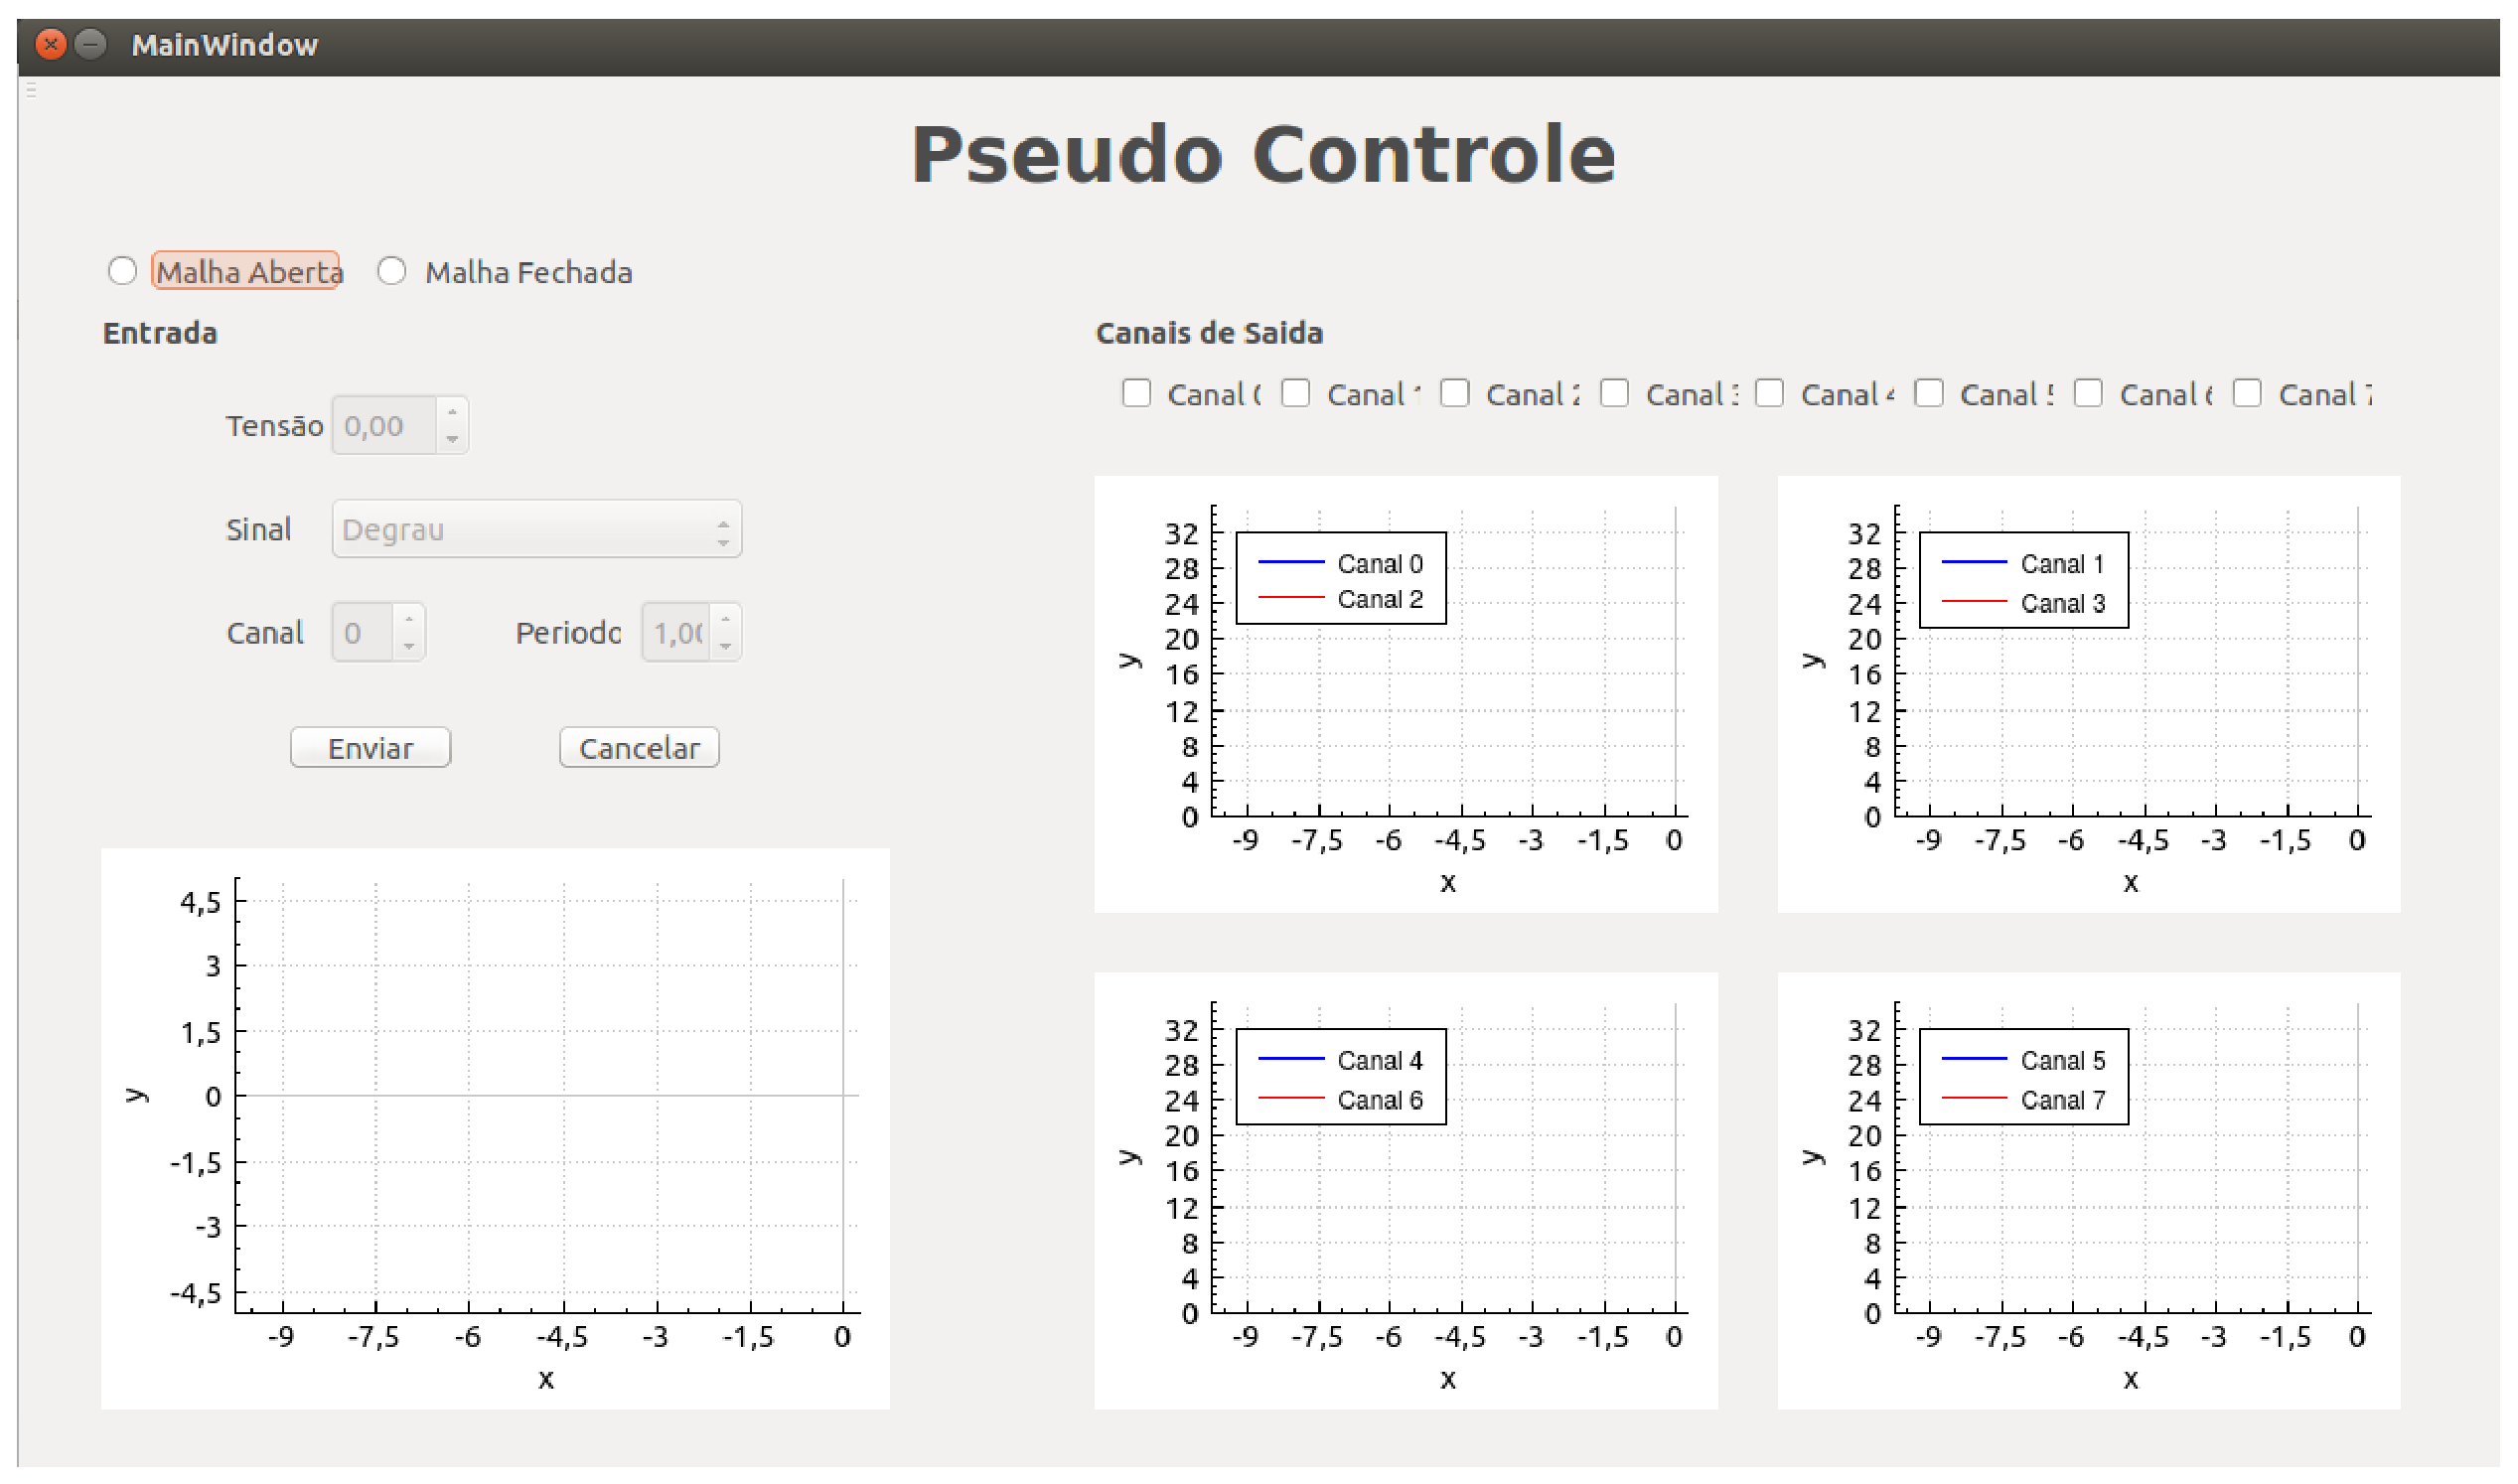
\includegraphics[width=0.9\textwidth]{prog-geral.eps}
\caption{Interface do programa de controle}
\label{Rotulo}
\end{figure}
\hspace{4ex}
Onde o gráfico principal que está localizado no canto inferior esquerdo apresenta o sinal enviado em tempo real. Os outros quatro gráficos à direita do gráfico principal apresentam as leituras dos possíveis oito canais disponíveis na placa. Entretanto, apenas dois obtinham informação relevante. No canal 0, a leitura do nível do tanque 1 e, no canal 1, a leitura do nível do tanque 2.


%\subsubsection{Subseções}

\newpage
\subsection{Sistema de tanques}
\hspace{4ex}
Pode-se observar através das leituras dos sensores como se deu o comportamento do nível dos tanques. Quando escolhido a malha aberta, a saída segue a entrada e se os dados recebidos não estiverem de acordo com a referência, só poderá ser corrigido quando a entrada é alterada. Dessa forma, o ajuste é feito manualmente. 

\begin{figure}[!h]
\centering
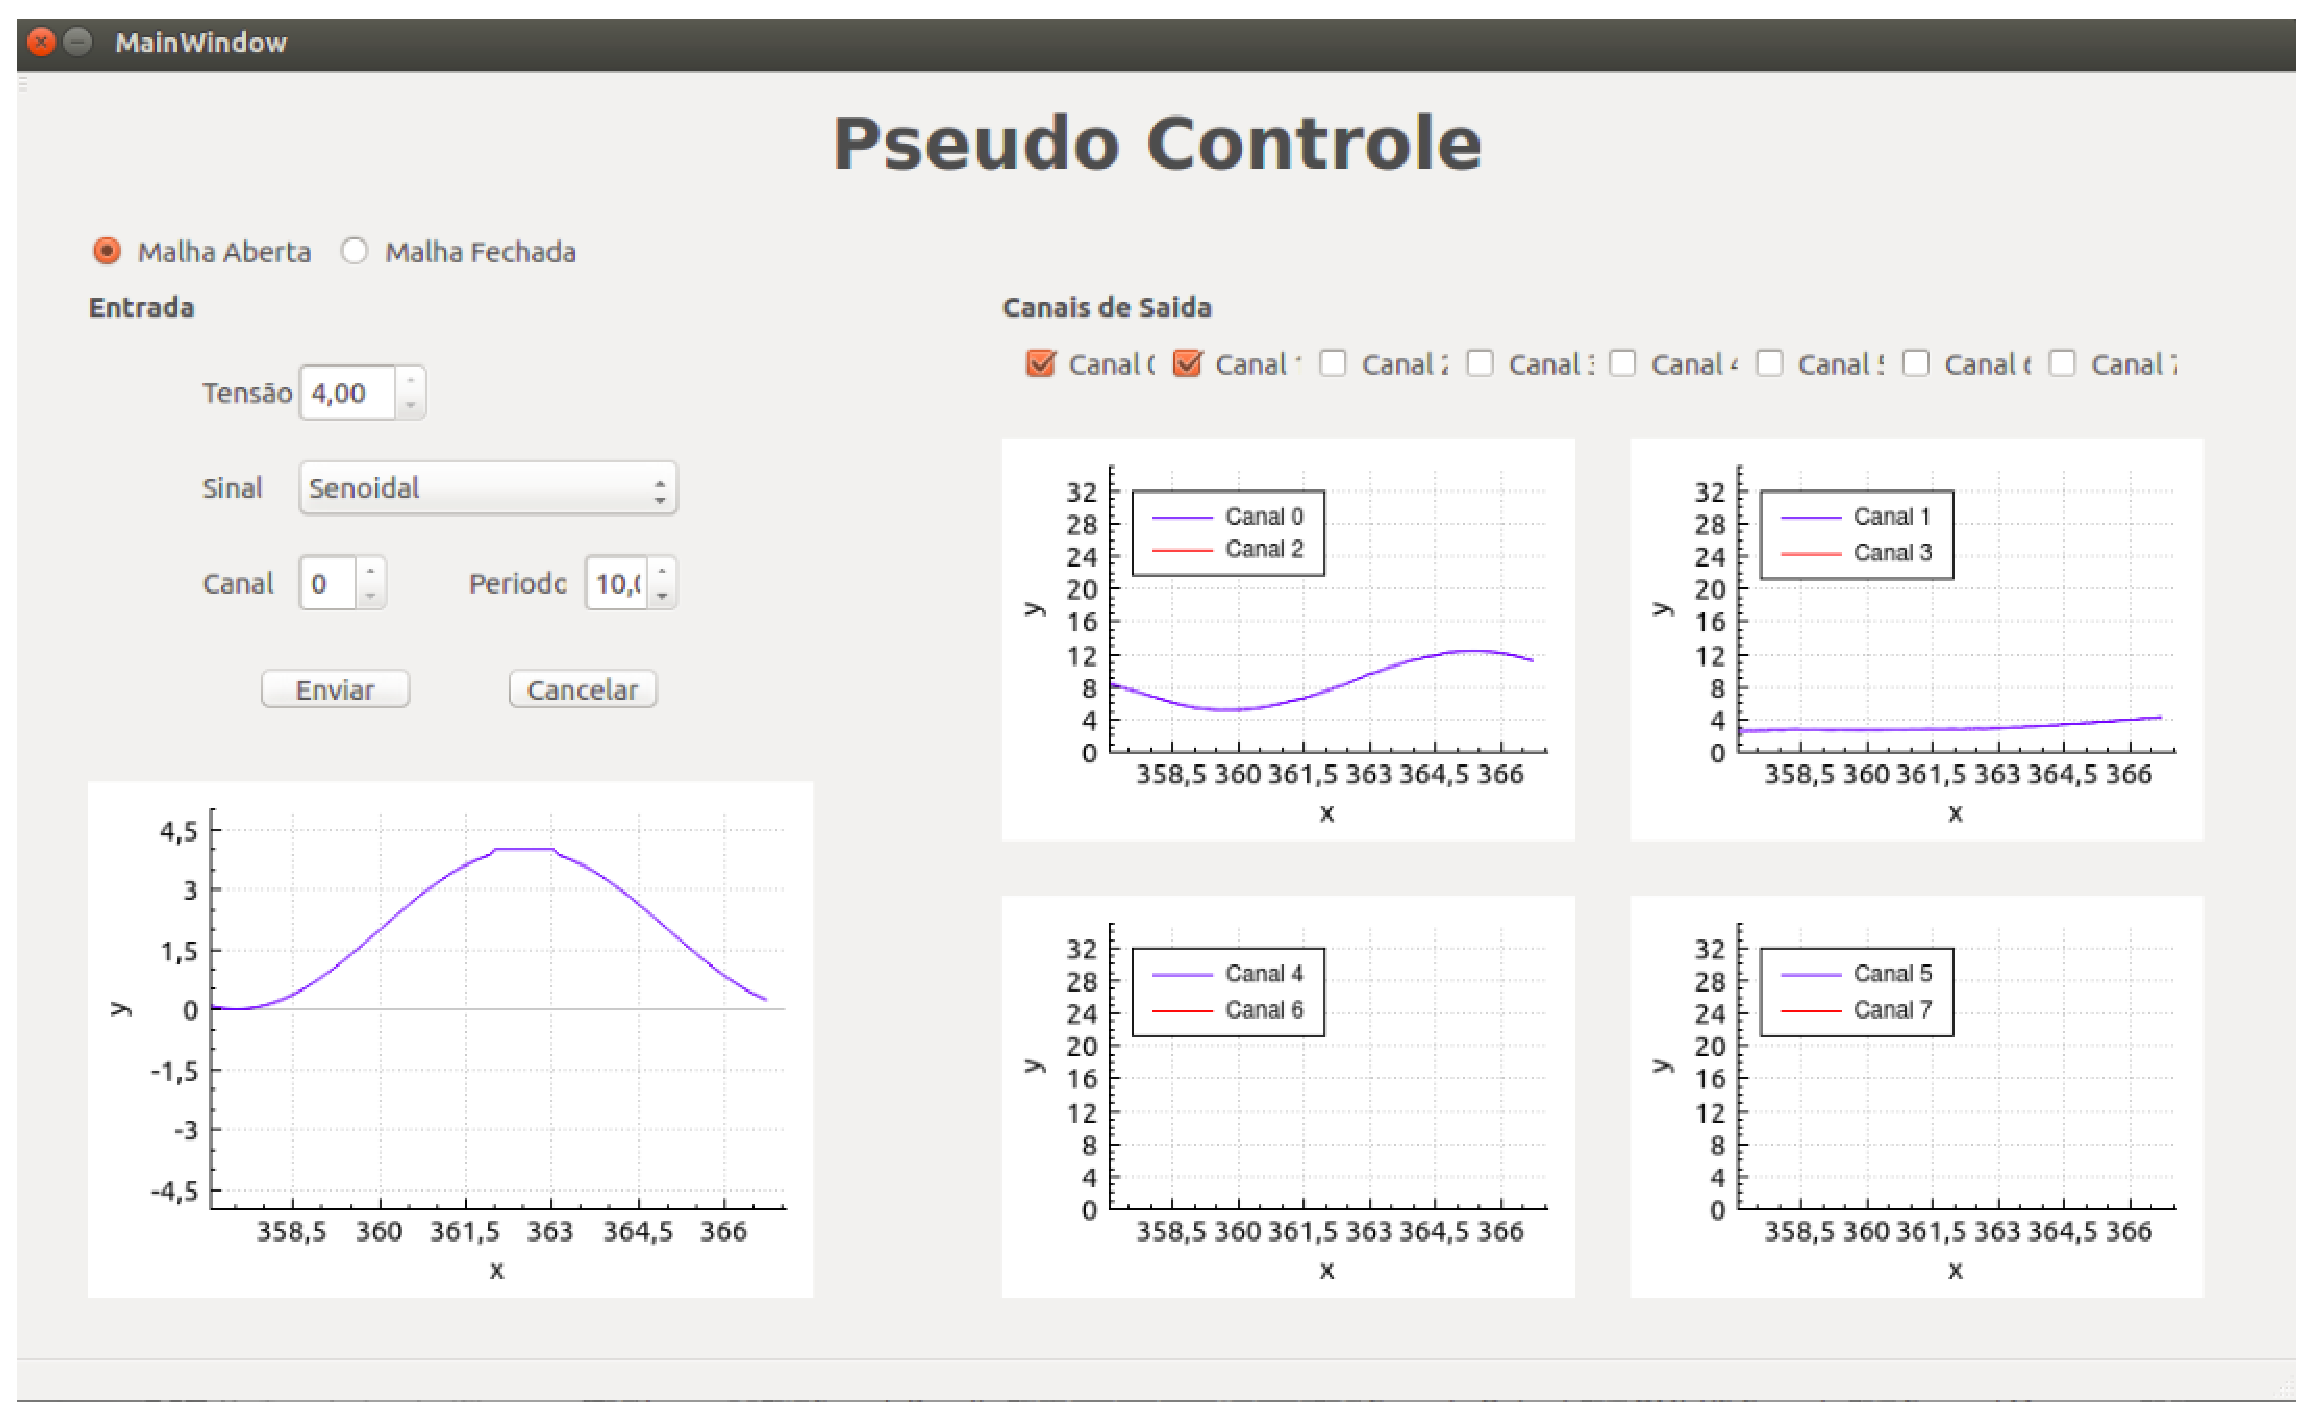
\includegraphics[width=0.8\textwidth]{maberta-sen-4.eps}
\caption{Sistem de controle para malha aberta com entrada senoidal}
\label{Entrada Senoidal - aberta}
\end{figure}
  
Na imagem acima pode-se ver que a resposta do sistema está deslocada em relação ao sinal de entrada. Enquanto a entrada está no seu ponto mínimo, na resposta o sinal está logo após o pico. 

\begin{figure}[!h]
\centering
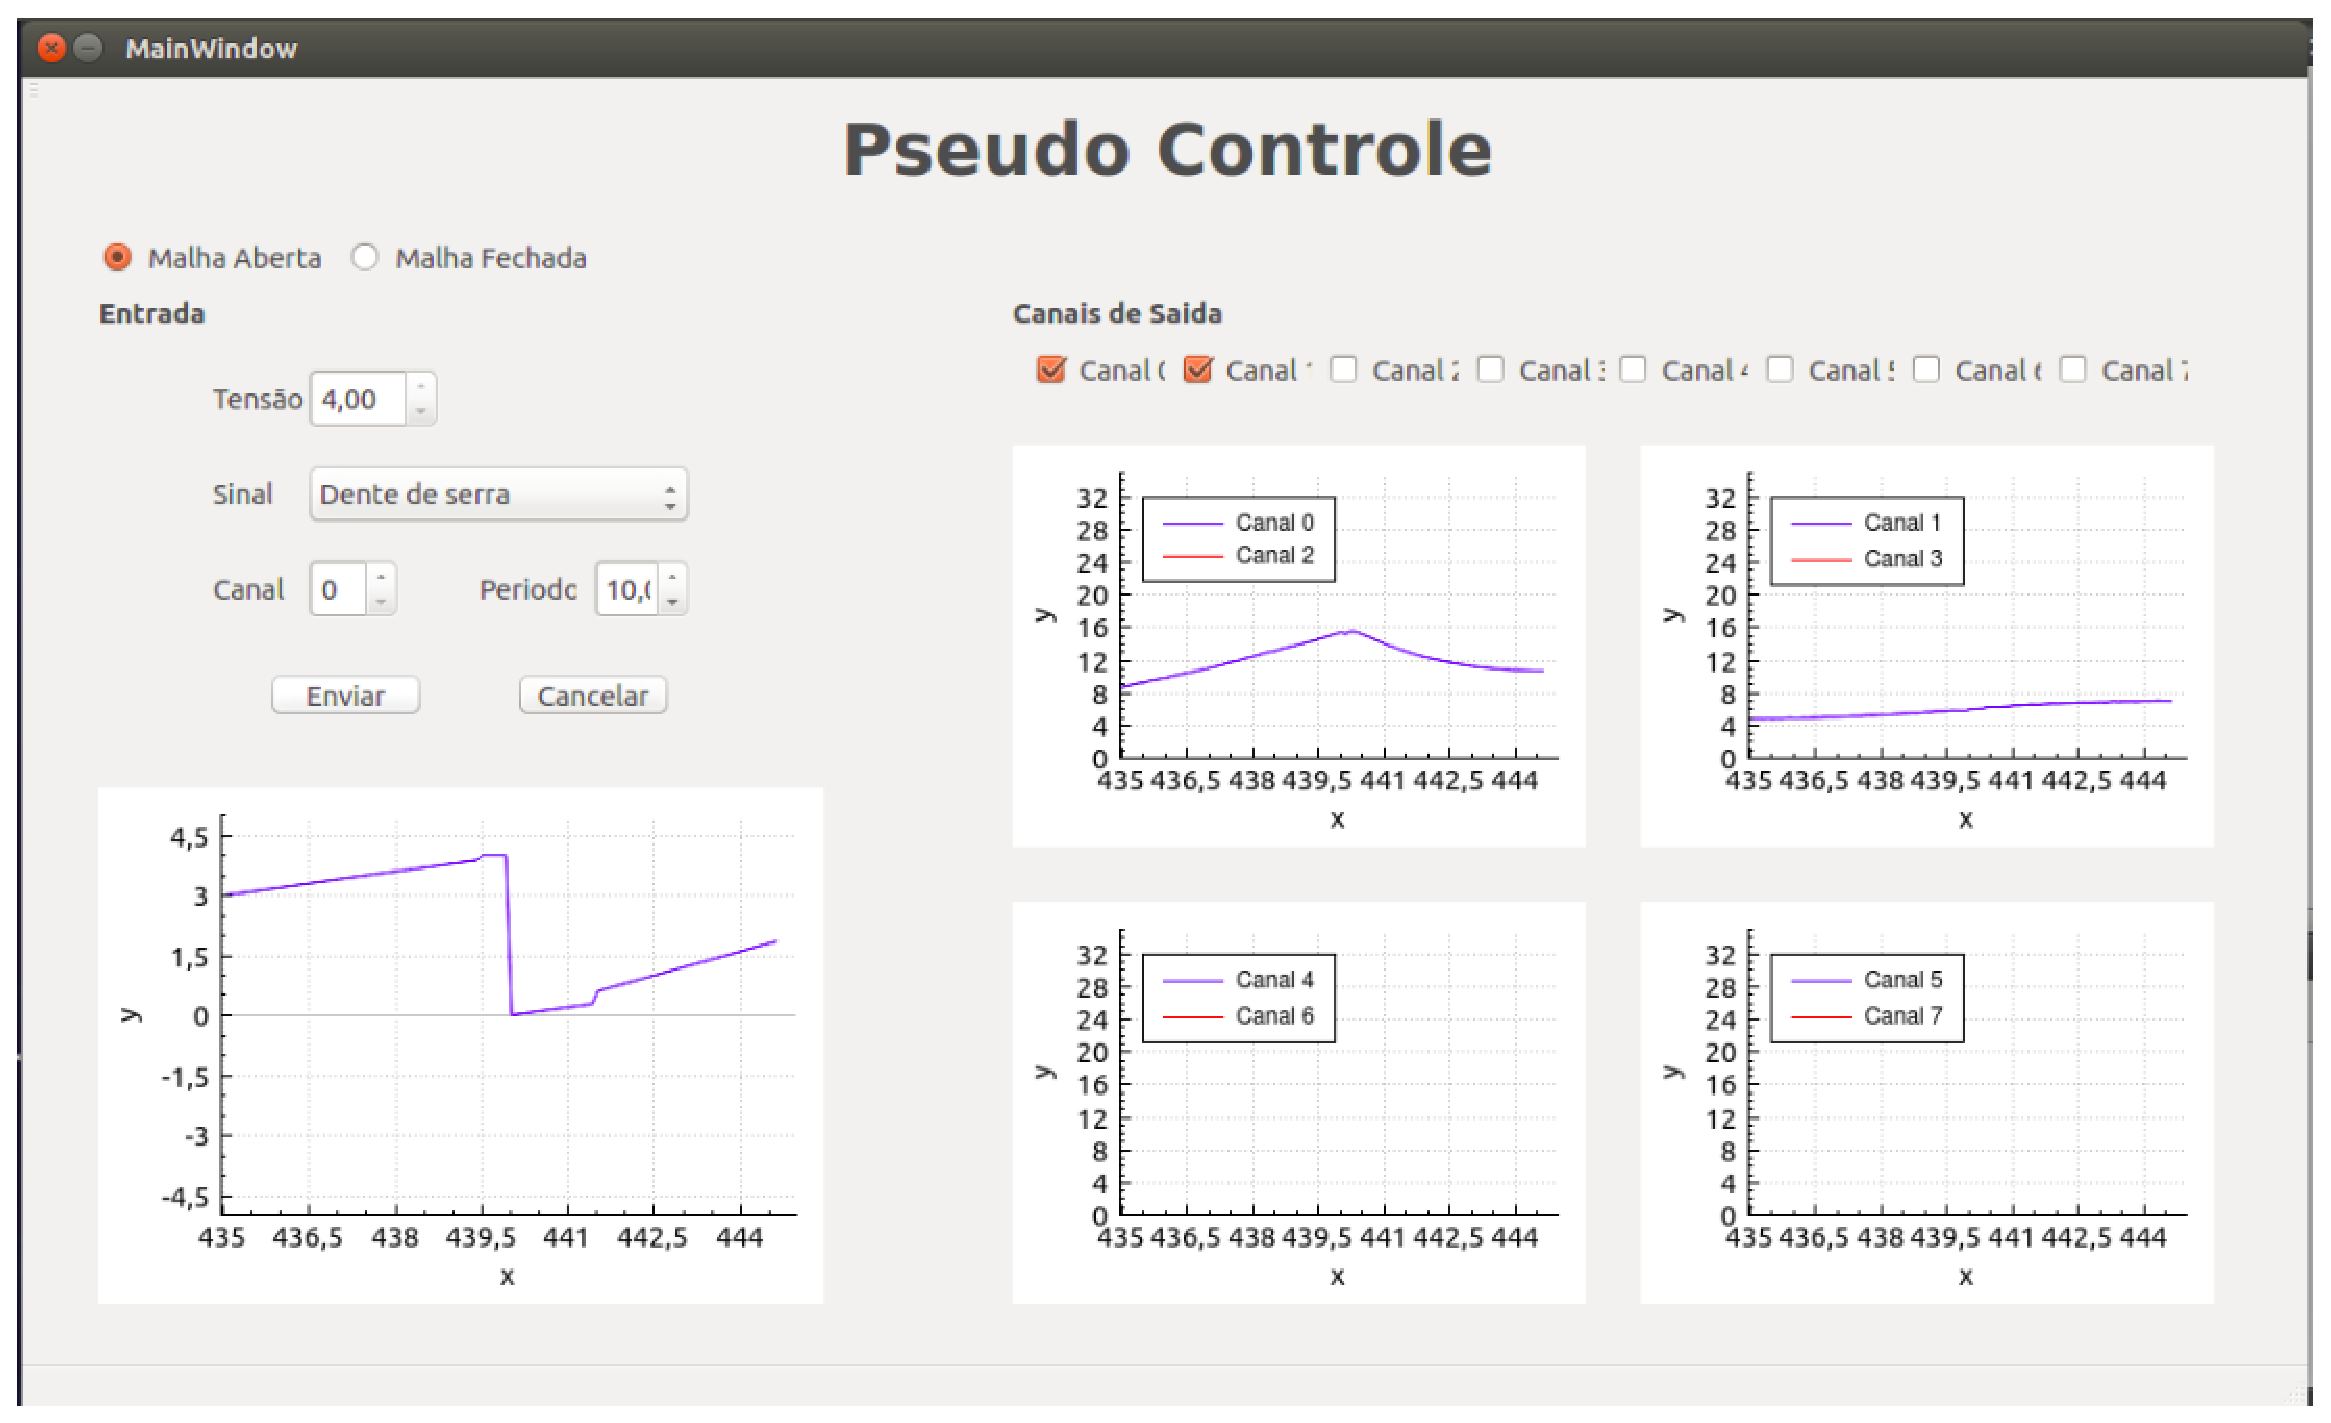
\includegraphics[width=0.8\textwidth]{maberta-serra-4.eps}
\caption{Sistem de controle para malha aberta com entrada dente de serra}
\label{Entrada Dente de Serra - aberta}
\end{figure}

\newpage
Já observando a resposta a um sinal dente de serra na figura 6, quando há a mudança brusca de valor quando se alcança a amplitude determinada na entrada, vê-se que o nível não segue o mesmo ritmo de mudança. O nível desce lentamente e dependendo do período, pode-se manter um certo nível.

Para o caso de malha fechada, o sistema vai tentar compensar o erro da referência. É o que se pode notar nos gráficos de saída. A figura 7 mostra que para uma entrada degrau em que a referência é 20cm, o sistema envia a tensão de 4 volts, ou seja, tensão máxima. O tanque alcança o nível, então para se manter no valor de referência, a tensão converge lentamente para uma tensão de equlíbrio.

\begin{figure}[!h]
\centering
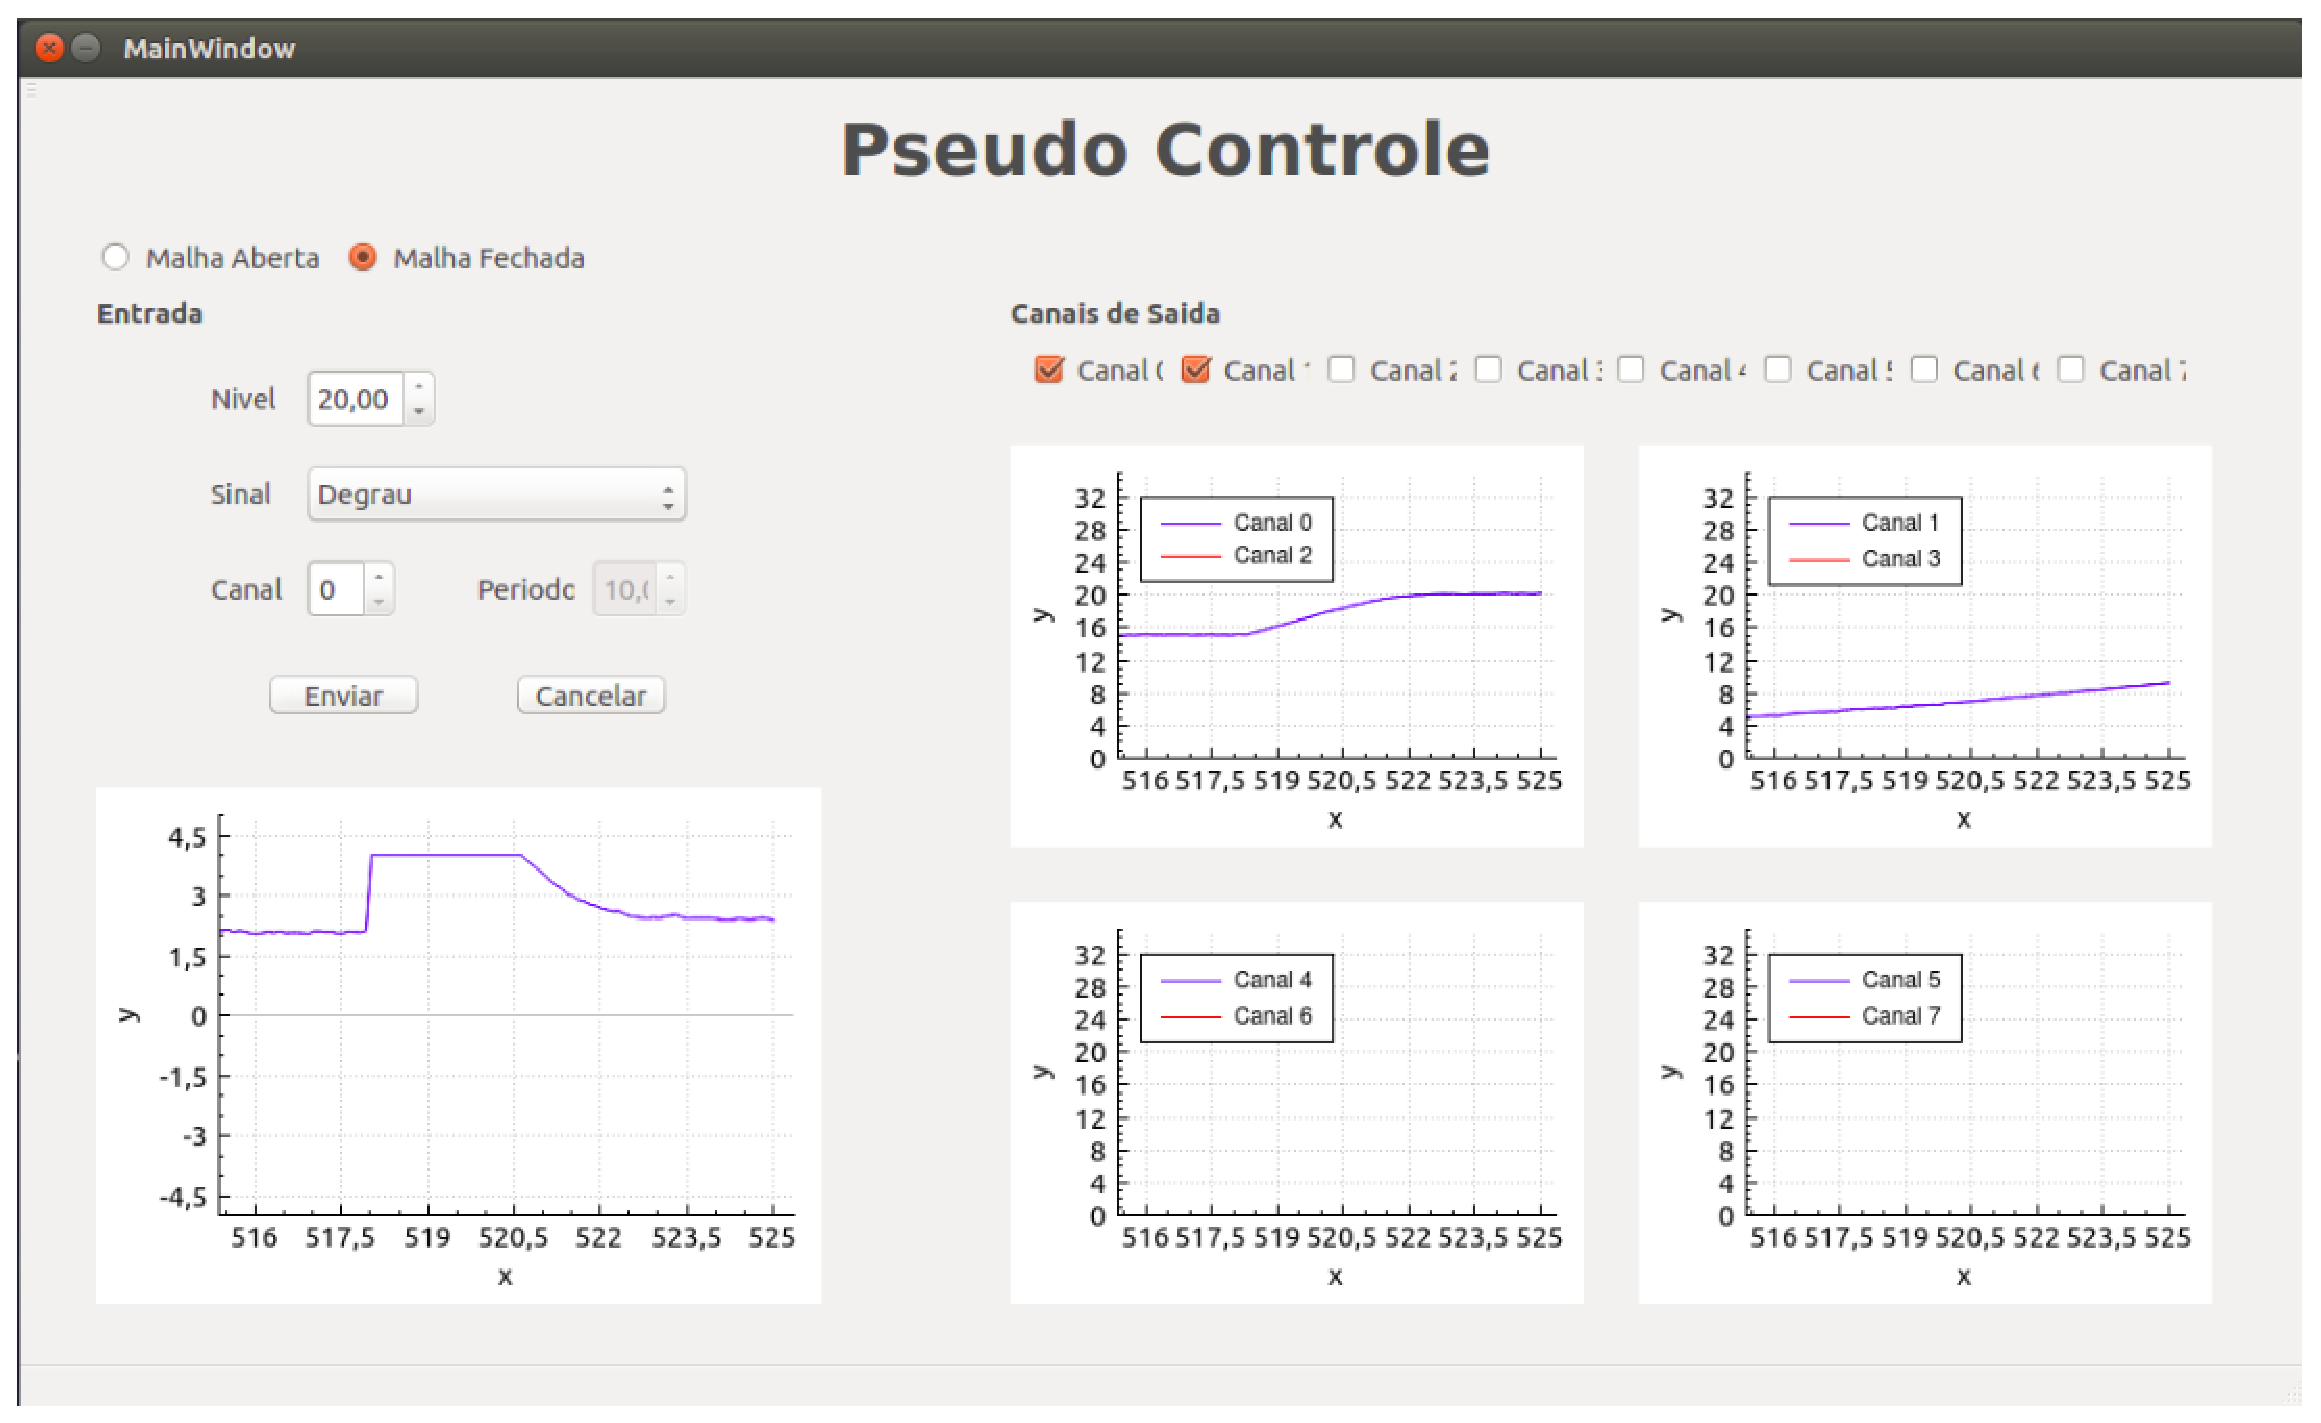
\includegraphics[width=0.8\textwidth]{mfechada-degrau-20.eps}
\caption{Sistem de controle para malha fechada com entrada degrau}
\label{Entrada Degrau - fechada}
\end{figure}



\begin{figure}[!h]
\centering
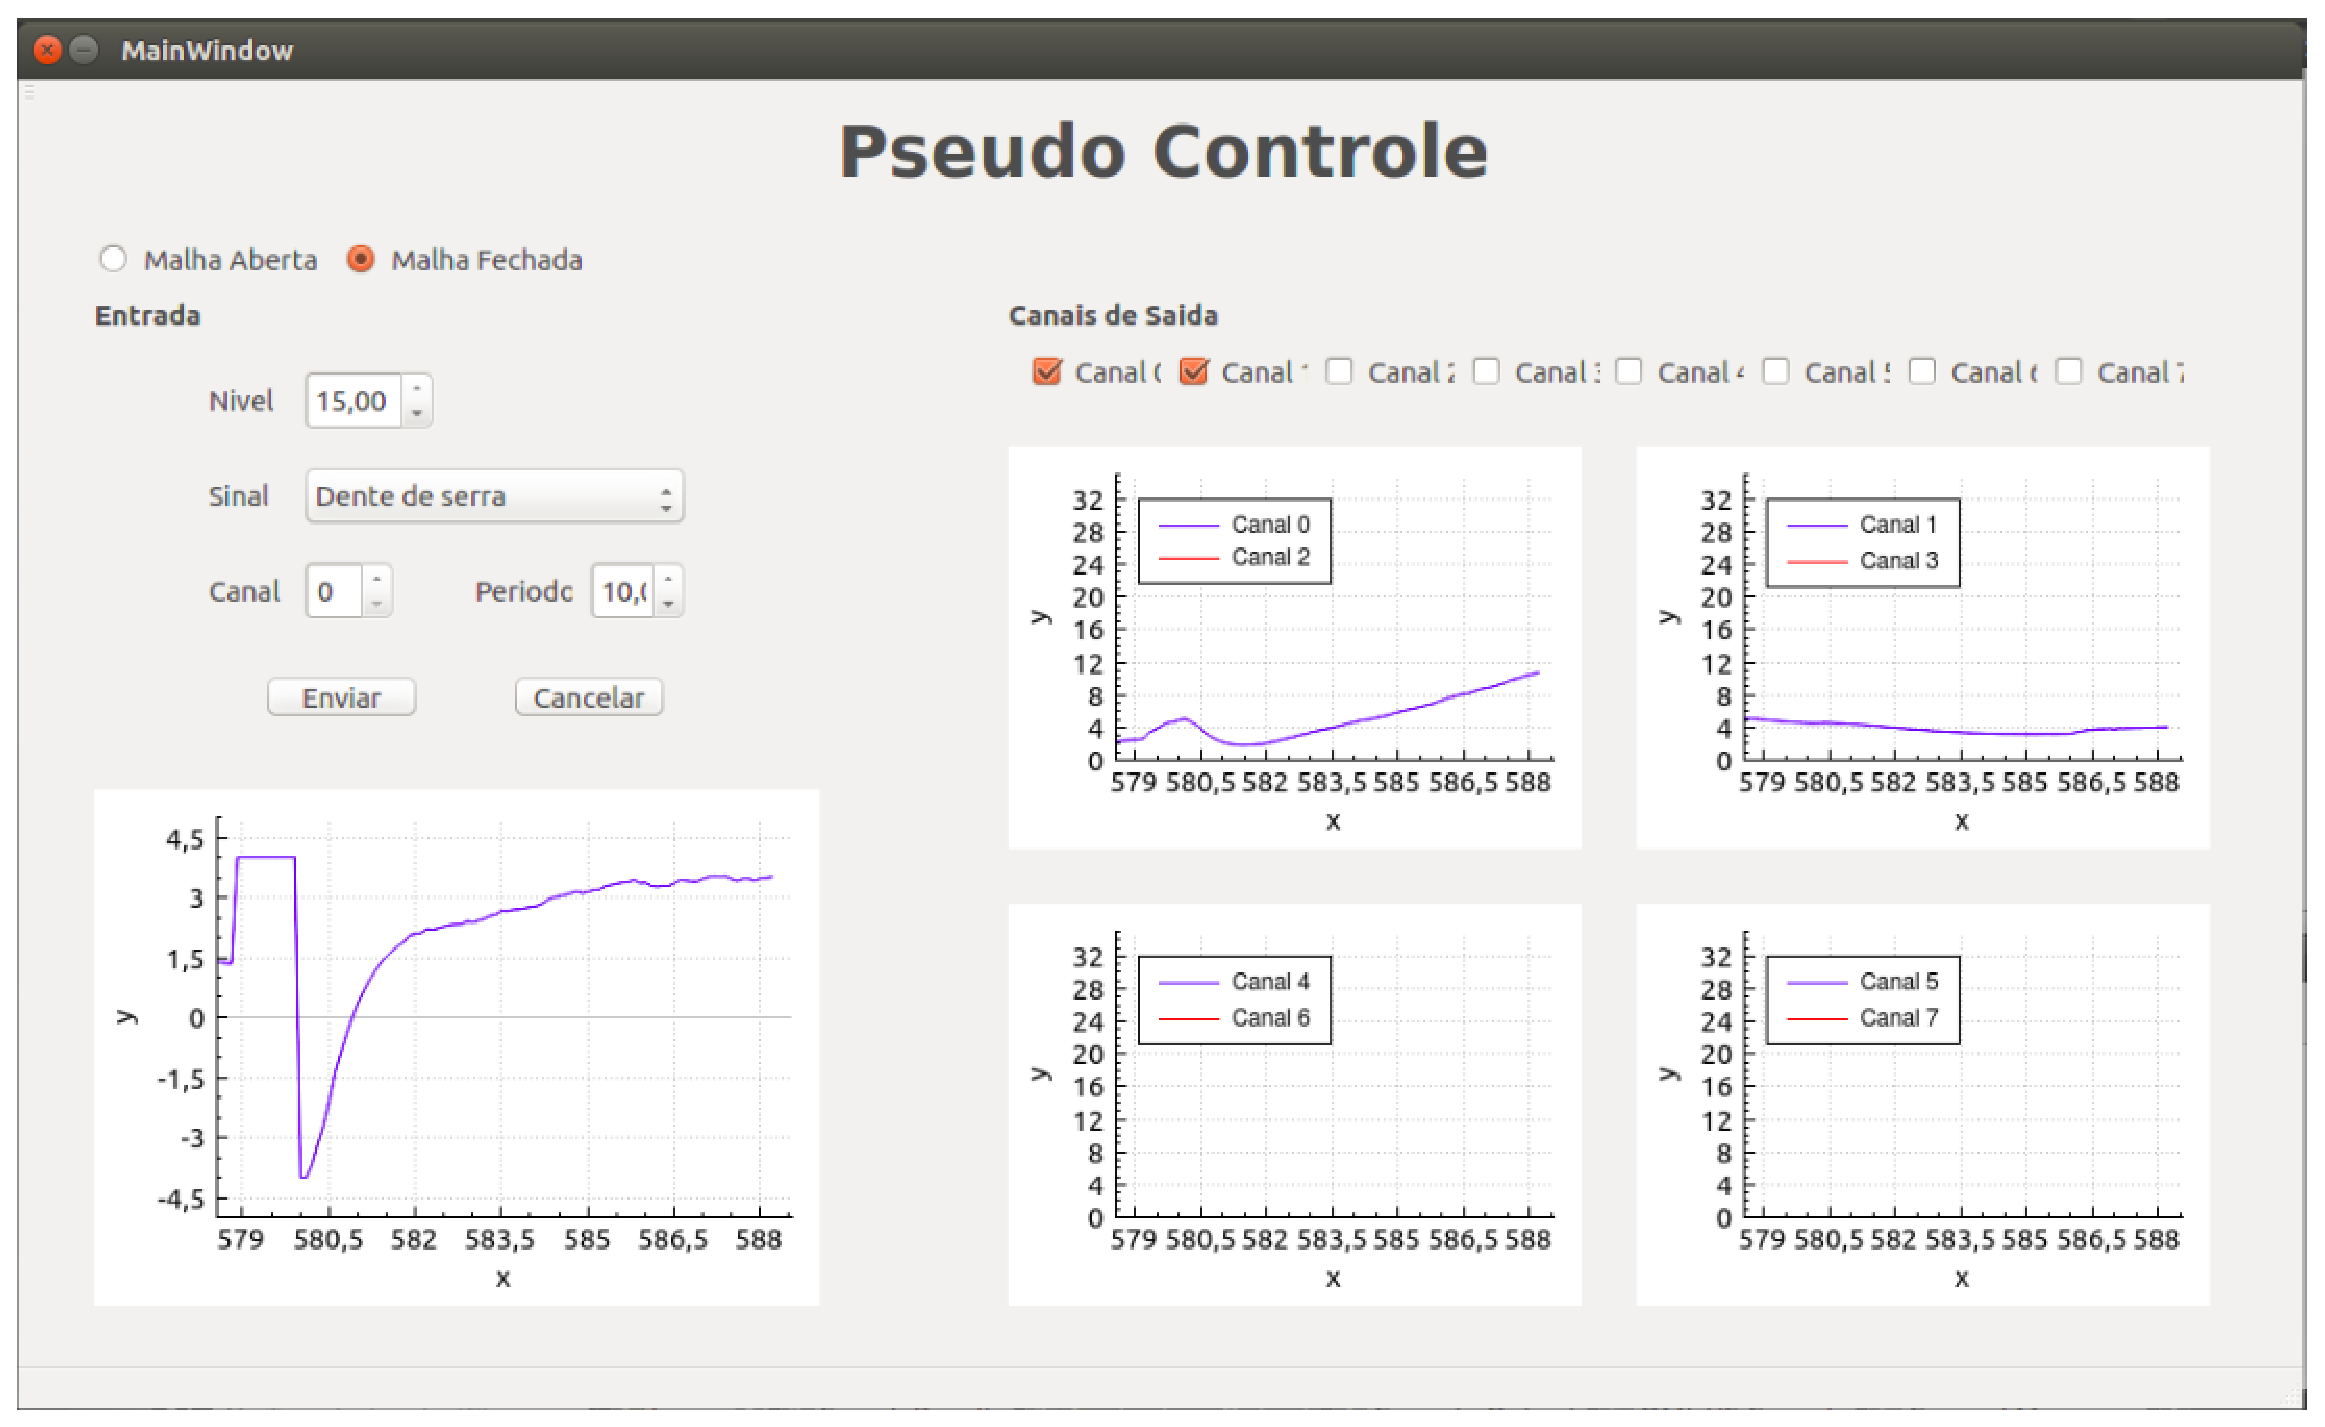
\includegraphics[width=0.8\textwidth]{mfechada-serra-15.eps}
\caption{Sistem de controle para malha fechada com dente de serra}
\label{Entrada Dente de serra - fechada}
\end{figure}

\begin{figure}[!h]
\centering
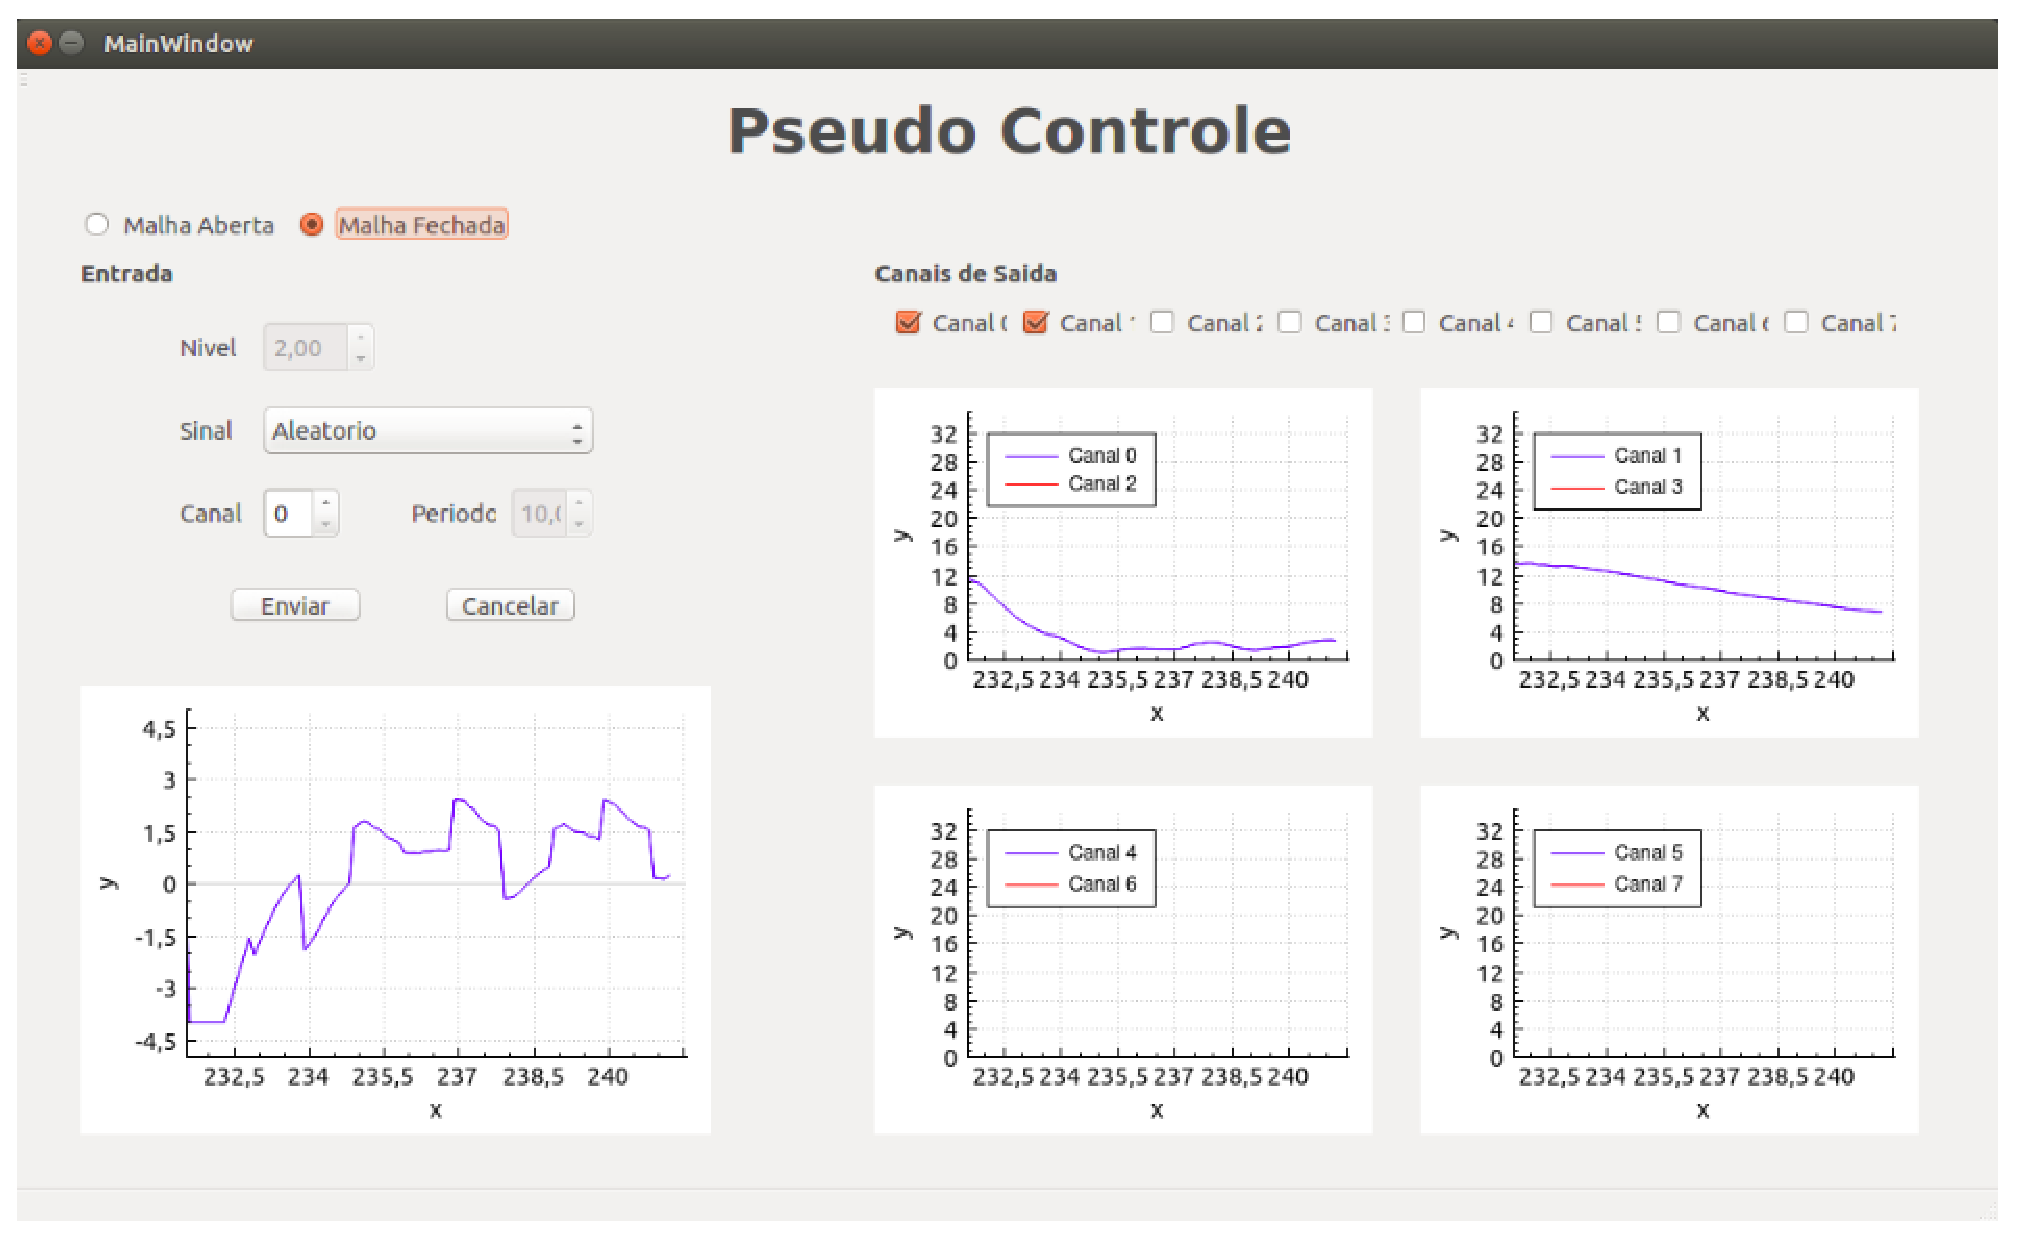
\includegraphics[width=0.8\textwidth]{mfechada-rand.eps}
\caption{Sistem de controle para malha fechada com aleatória}
\label{Entrada aleatória - fechada}
\end{figure}


\newpage

%%%%%%%%%% CONCLUSÃO %%%%%%%%%%%%%%%

\thispagestyle{main}

\section{CONCLUSÃO}


\hspace{4ex}De acordo com os resultados obtidos, pode-se concluir que na malha fechada, o controlador consegue rastrear bem o degrau, para os demais sinais, esse rastreamento só é possível se a variação do sinal for mais lenta que a constante de tempo do sistema. Enquanto que na malha aberta, é importante ressaltar que o sinal dificilmente ficará no valor calculado teoricamente, devido a interferência de fatores externos e internos, como por exemplo a temperatura, funcionamento da bomba e ajustes dos sensores da planta.

Além disso, o controlador utilizado na malha fechada calcula o erro do nível do tanque e soma com a tensão necessária para chegar na altura desejada pelo usuário, dessa forma, o erro faz o papel de acelerador do sistema, fazendo com que um determinado nível seja alcançado rapidamente, diferentemente do caso em que se utiliza apenas o valor do erro onde o valor desejado pode não ser alcançado.

\newpage

%%%%%%%% REFERÊNCIAS %%%%%%%%%%%%%%%%%

% Referências bibliogáficas (geradas automaticamente)
\addcontentsline{toc}{chapter}{Referências bibliográficas}
\bibliography{bib/bibliografia}

\appendix

%Apêndice A
\include{apendice}

\end{document}
